% -*- coding: utf-8 -*-
% ============================================================
%  Poster: 基于深度学习的加密流量分类
%  Compile: xelatex poster.tex
% ============================================================
\documentclass[25pt, a0paper, portrait, margin=20mm, innermargin=15mm,
blockverticalspace=15mm, colspace=15mm, subcolspace=8mm]{tikzposter}

\usepackage{ctex}
\usepackage{graphicx}
\usepackage{booktabs}
\usepackage{enumitem}
\usepackage{amsmath}
\usepackage{hyperref}
\usepackage{xcolor}

% ── Theme ──
\usetheme{Board}
\usecolorstyle{Australia}

\colorlet{blocktitlebgcolor}{blue!60!black}
\colorlet{blockbodybgcolor}{white}
\colorlet{innerblocktitlebgcolor}{blue!10}
\colorlet{innerblockbodybgcolor}{white}

% ── Title style ──
\settitle{
    \centering
    \color{white}
    \vspace{1cm}
    {\bfseries \Huge 基于深度学习的加密网络流量分类研究}\\[1cm]
    {\LARGE Encrypted Traffic Classification via CNN/LSTM with Packet-Length Sequences}\\[1.5cm]
    {\Large 上海交通大学 \quad CS3611 计算机网络 \quad 期末项目}\\[0.5cm]
    {\large \today}
}

% ── Block spacing ──
\addtolength{\topmargin}{-15mm}

\begin{document}

\maketitle

% ═══════════════════════════════════════════════════════════
\begin{columns}

% ── LEFT COLUMN ──
\column{0.32}

\block{研究背景与动机}{
    \textbf{问题}：网络流量加密（TLS/HTTPS）使得传统的深度包检测（DPI）失效，
    基于端口和载荷特征的分类方法不再适用。

    \textbf{关键观察}：虽然载荷已加密，但\textbf{包长序列}（packet-length sequence）
    仍保留了应用层行为的统计特征——不同应用（视频、聊天、文件传输等）
    具有不同的流量模式和包长分布。

    \textbf{研究目标}：
    \begin{itemize}[nosep]
        \item 利用 TCP 包长序列进行加密流量分类
        \item 比较 CNN 与 LSTM 在此任务上的表现
        \item 探索类别粒度（3/4/5类）和序列长度对分类效果的影响
    \end{itemize}

    \textbf{数据集}：ISCX NonVPN 数据集，包含 110 个 PCAP 文件，
    涵盖 AIM、Facebook、Skype、YouTube、Netflix 等多种应用，
    按应用类型划分为 7 个细分类别。
}

\block{数据处理流程}{
    \begin{enumerate}[nosep]
        \item \textbf{PCAP 解析}：使用 Scapy 读取每个 TCP 流的包长序列
        \item \textbf{流过滤}：丢弃包数 $< \text{min\_packets}$ 的短流（默认 $\geq 5$）
        \item \textbf{特征构建}：取每条流前 $N$ 个包的包长，除以 MTU (1500) 归一化到 $[0, 1]$
        \item \textbf{去重}：每 PCAP 内部去除特征向量完全相同的流
        \item \textbf{类别映射}：支持 tcp3/4/5/7/8 五种类别合并方案
    \end{enumerate}

    \begin{center}
        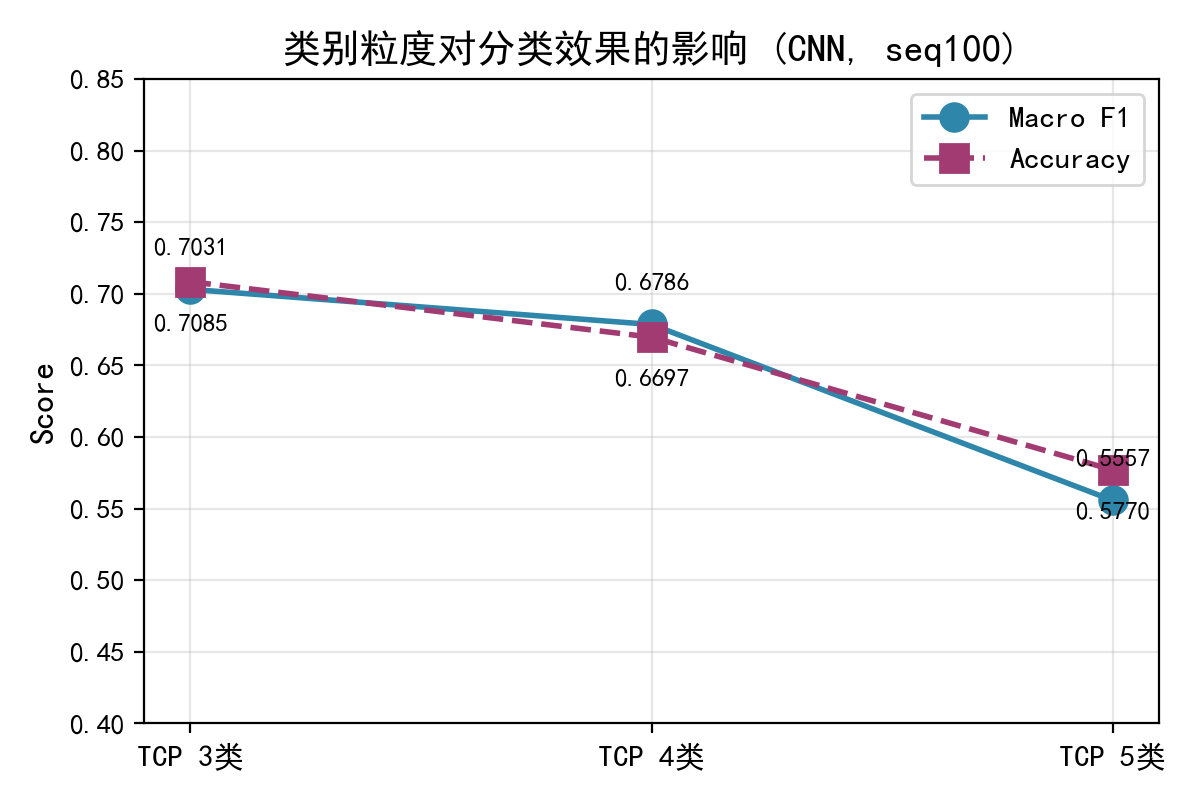
\includegraphics[width=0.75\linewidth]{poster_class_count.png}
        \innerblock{类别映射方案}{
            \begin{tabular}{c|l}
                \textbf{Scheme} & \textbf{类别合并} \\
                \hline
                tcp5class & Comm / Email / Media / VideoCall / File \\
                tcp4class & Comm / Email / Media+VideoCall / File \\
                tcp3class & Comm+Email / Media+VideoCall / File \\
            \end{tabular}
        }
    \end{center}

    最终生成数据集：4901 条流，分别按 3/4/5 类和 seq32/64/100 保存。
}

% ── MIDDLE COLUMN ──
\column{0.36}

\block{模型架构}{
    \textbf{CNN1D 分类器}：三阶段 1D 卷积网络
    \begin{itemize}[nosep]
        \item Conv1D(1→32, k=3) → BatchNorm → GELU → MaxPool(2)
        \item Conv1D(32→64, k=3) → BatchNorm → GELU → MaxPool(2)
        \item Conv1D(64→128, k=3) → BatchNorm → GELU → AdaptiveAvgPool
        \item Flatten → Linear(128→64) → GELU → Dropout(0.3) → Linear(64→N)
    \end{itemize}

    \textbf{LSTM 分类器}：双层单向 LSTM
    \begin{itemize}[nosep]
        \item LSTM(input=1, hidden=128, layers=2, dropout=0.2)
        \item Mean pooling over valid timesteps
        \item Linear(128→64) → ReLU → Dropout(0.3) → Linear(64→N)
    \end{itemize}

    \textbf{训练配置} (统一)：
    \begin{itemize}[nosep]
        \item Optimizer: AdamW (lr=$5\times10^{-5}$, weight\_decay=$10^{-4}$)
        \item Scheduler: CosineAnnealingLR
        \item Loss: CrossEntropyLoss + Class-balanced WeightedRandomSampler
        \item Epochs: 100, Batch Size: 64
        \item Train/Val Split: 80/20, stratified
    \end{itemize}
}

\block{实验结果：CNN vs LSTM}{
    \begin{center}
        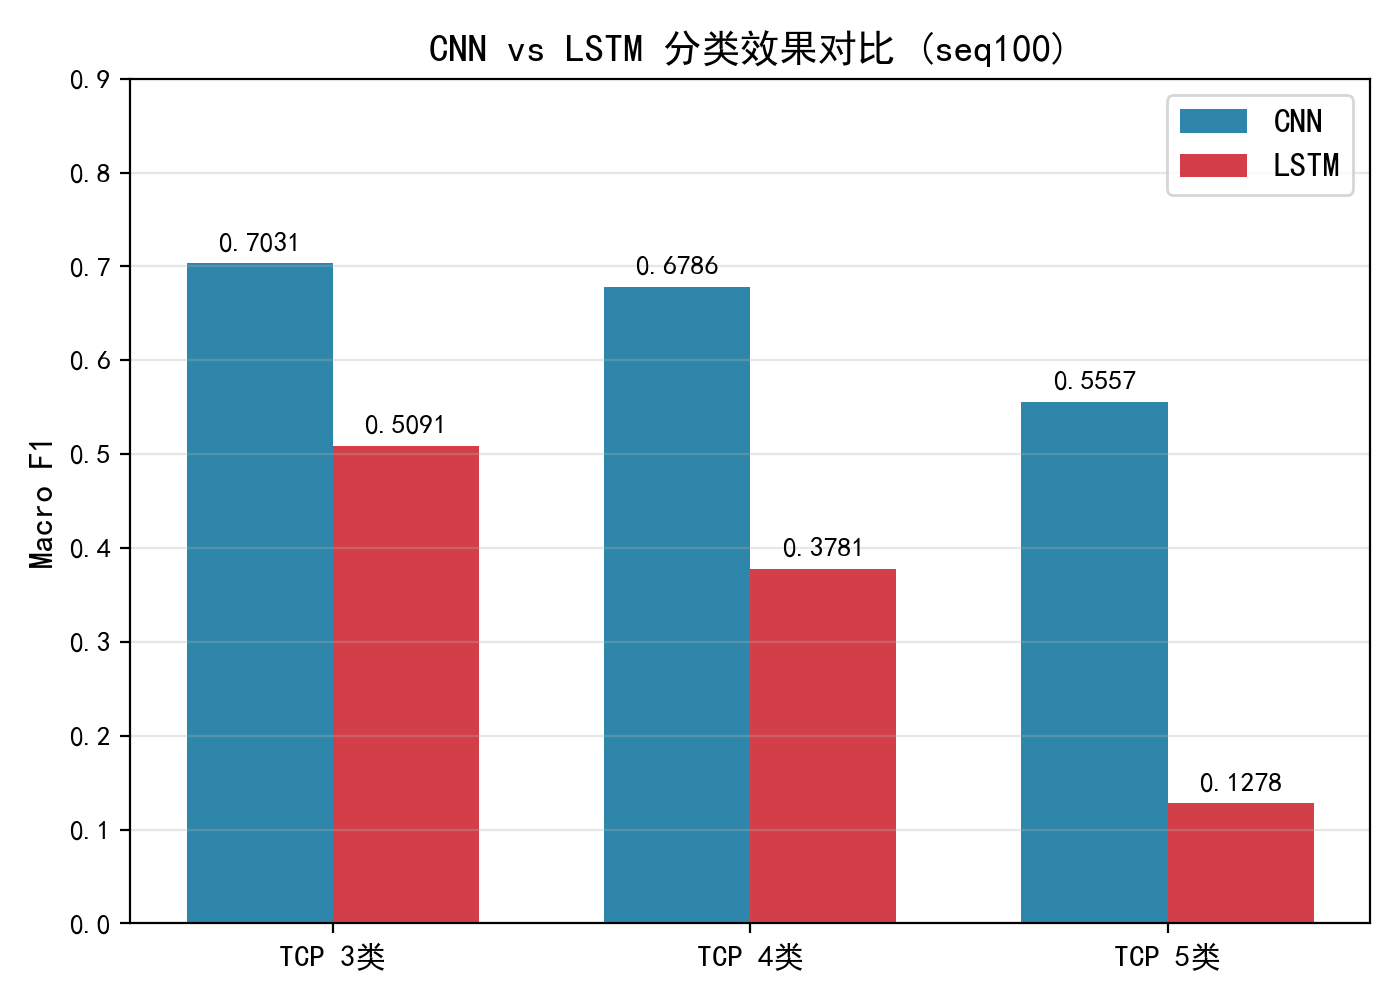
\includegraphics[width=0.82\linewidth]{poster_cnn_vs_lstm.png}
    \end{center}

    CNN 在所有类别方案上显著优于 LSTM：
    \begin{itemize}[nosep]
        \item 3 类：CNN 0.703 $\gg$ LSTM 0.509（差距 0.194）
        \item 4 类：CNN 0.679 $\gg$ LSTM 0.378（差距 0.301）
        \item 5 类：CNN 0.556 $\gg$ LSTM 0.128（差距 0.428）
    \end{itemize}

    \innerblock{分析}{
        LSTM 参数量更大（$\sim$200K vs $\sim$80K），在小数据集上容易过拟合。
        CNN 的局部感受野更适合捕获包长序列的短距离模式。
        类别越多，LSTM 退化越严重（5 类时几乎随机）。
    }
}

% ── RIGHT COLUMN ──
\column{0.32}

\block{实验结果：序列长度影响}{
    \begin{center}
        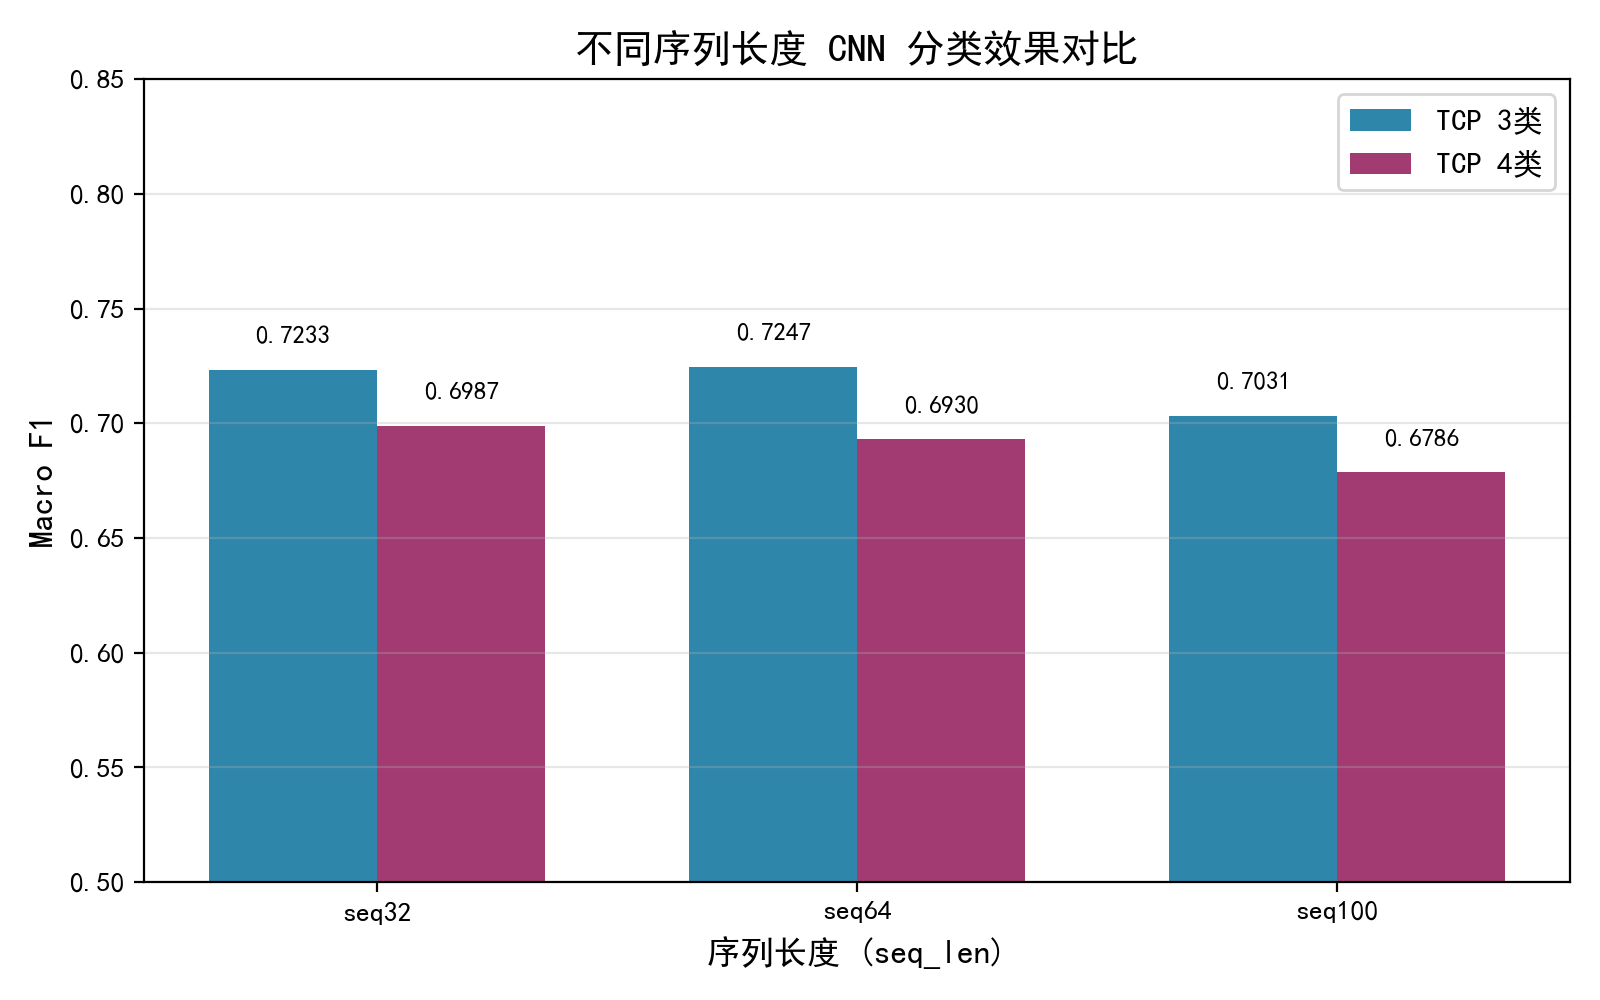
\includegraphics[width=0.85\linewidth]{poster_seq_comparison.png}
    \end{center}

    \textbf{关键发现}：
    \begin{itemize}[nosep]
        \item seq32 和 seq64 性能接近，均优于 seq100
        \item 更长的序列引入更多噪声而非有用信息
        \item \textbf{最佳结果}：tcp3class + seq64 → Macro F1 = \textbf{0.7247}
    \end{itemize}
}

\block{最佳模型详细结果}{
    \textbf{方案}：tcp3class, CNN, seq64\\
    \textbf{Macro F1}：0.7247 \quad \textbf{Accuracy}：0.7288

    \begin{center}
        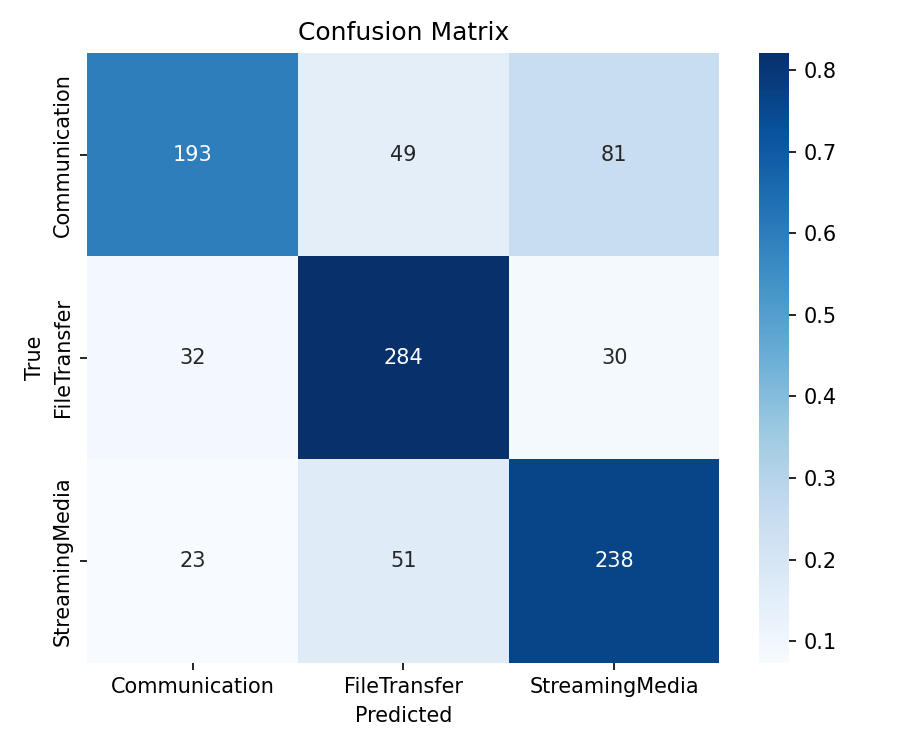
\includegraphics[width=0.72\linewidth]{poster_best_confusion.png}
    \end{center}

    \begin{tabular}{lrrr}
        \toprule
        \textbf{类别} & \textbf{Precision} & \textbf{Recall} & \textbf{F1} \\
        \midrule
        Communication & 0.778 & 0.598 & 0.676 \\
        FileTransfer   & 0.740 & 0.821 & 0.778 \\
        StreamingMedia & 0.682 & 0.763 & 0.720 \\
        \bottomrule
    \end{tabular}

    Communication 类存在一定混淆（recall 较低），可能与 Email 混入后
    包长模式接近聊天/音频有关；FileTransfer 区分度最好。
}

\block{结论与展望}{
    \begin{itemize}[nosep]
        \item \textbf{CNN $\gg$ LSTM}：在包长序列分类任务上 CNN 更具优势
        \item \textbf{seq32/64 最优}：过长的序列引入噪声，32--64 包足以捕获应用特征
        \item \textbf{3 类效果最佳}：类别粒度越细，类间混淆越大
        \item \textbf{后续工作}：
            \begin{itemize}[nosep]
                \item 引入包间间隔（IAT）作为额外特征
                \item 探索滑动窗口数据增强对 CNN 的提升
                \item 在 VPN 数据集上验证泛化能力
                \item 实现实时在线分类代理
            \end{itemize}
    \end{itemize}
}

\end{columns}

\end{document}
